%% LyX 2.3.3 created this file.  For more info, see http://www.lyx.org/.
%% Do not edit unless you really know what you are doing.
\documentclass[english]{beamer}
\usepackage{lmodern}
\renewcommand{\sfdefault}{lmss}
\renewcommand{\ttdefault}{lmtt}
\usepackage[T1]{fontenc}
\usepackage{mathtools}
\usepackage{amsmath}
\usepackage{amssymb}
\usepackage{graphicx}

\makeatletter
%%%%%%%%%%%%%%%%%%%%%%%%%%%%%% Textclass specific LaTeX commands.
% this default might be overridden by plain title style
\newcommand\makebeamertitle{\frame{\maketitle}}%
% (ERT) argument for the TOC
\AtBeginDocument{%
  \let\origtableofcontents=\tableofcontents
  \def\tableofcontents{\@ifnextchar[{\origtableofcontents}{\gobbletableofcontents}}
  \def\gobbletableofcontents#1{\origtableofcontents}
}

%%%%%%%%%%%%%%%%%%%%%%%%%%%%%% User specified LaTeX commands.
\usetheme{Warsaw}
% or ...

\setbeamercovered{transparent}
% or whatever (possibly just delete it)

\makeatother

\usepackage{babel}
\begin{document}
\title{Circular Coordinates under Different Cost Functions}
\subtitle{Group 8 Project}
\institute{ICERM August 2019}
\date{Applied Mathematical Modeling with Topological Techniques}
\makebeamertitle
\begin{frame}{Problem Setup}
\begin{itemize}
\item Given a simplicial complex $K$ from the dataset $X$, we can
consider the homology and cohomology with a fixed coefficient field
$\Bbbk$.
\item Homology and boundary operator: $\partial:C_{k}(K)\rightarrow C_{k-1}(K)$.
e.g. $\partial[a,b,c]=[a,b]+[b,c]+[c,a]$
\item Cohomology and coboundary operator: $\delta:C^{k}(K)\rightarrow C^{k+1}(K)$.
e.g. \small{$\delta\left[\begin{array}{c}
a\mapsto1\\
b\mapsto0\\
c\mapsto0
\end{array}\right]=-[a,b]^{*}+[c,a]^{*}$ with $[a,b]^{*}=\left[\begin{array}{c}
ab\mapsto1\\
bc\mapsto0\\
ca\mapsto0
\end{array}\right]$.}
\item \textbf{Intuition:} If you think of boundary operators as ``derivation'',
then the coboundary operator is like ``anti-derivation''.
\end{itemize}
\end{frame}

\begin{frame}
\begin{itemize}
\item \textbf{Theorem} (\textit{Circular Coordinates}): Given a $[f]\in H^{1}_{\mathbb{Z}}(X)$, $f$ can
be made into a function $X\rightarrow S^{1}$. This \textbf{circular
coordinate} can be found through the optimization problem $\min_{z\in C^{0}(X)}\|f-\delta z\|_{L^{2}}$.\\
%
\end{itemize}
%\begin{itemize}
%\item \textbf{Problem} (New): How about we change the cost function $\|x\|_{L^{2}}\coloneqq(\sum_{i}x_{i}^{2})^{1/2}$
%\begin{itemize}
%\item $\|x\|_{L^{1}}\coloneqq(\sum_{i}|x_{i}|)$ L1-norm\\
%It may introduce sparsity across coordinates instead of smoothness.
%\item $(1-\lambda)\|x\|_{L^{1}}+\lambda\|x\|_{L^{2}}$ elastic net\\
%It may find a balance between L1 and L2 norms.
%\item $\|x\|_{L^{1}}+\lambda\|x\|_{L^{p}}$\\
%It may produces some other kind of smoothness.
%\item Localized penalty. Only take a penalty norm for some subvector of
%$x$.
%\item In addition, we can penalize not only $x=f-\delta z$ but also
%\begin{itemize}
%\item $x=\delta z$ (minimize edits?)
%\item $x=z$ or $x=z\text{ mod }1$ (smaller values for functions as $X\rightarrow S^{1}$?)
%\end{itemize}
%\end{itemize}
%\end{itemize}
\begin{itemize}
	\item \textbf{Problem} (New): How about adding a regularization term $\mathcal{R}(x)$ on $x=f - \delta z$?
	\begin{itemize}
		\item $\|x\|_{L^{2}}\coloneqq(\sum_{i}|x_{i}|)$ L2-norm\\		
		\item $\|x\|_{L^{1}}\coloneqq(\sum_{i}|x_{i}|)$ L1-norm\\
		It may introduce sparsity across coordinates instead of smoothness.
		\item $(1-\lambda)\|x\|_{L^{1}}+\lambda\|x\|_{L^{2}}$ elastic net\\
		It may find a balance between L1 and L2 norms.
	\end{itemize}
\end{itemize}

\begin{itemize}
	\item Generic matrix optimization without Jacobian estimate: Slow and inefficient.
	\item Matrix optimization using Gradient Descent with Jacobian.
\end{itemize}
\end{frame}
%
\begin{frame}{Optimization Problem: Gradient Descent}
\begin{itemize}
\item Example 1: Annulus, L2 norm ($\|f-\delta z\|_{2}$) and L1 norm ($\|f-\delta z\|_{1}$)\\
\begin{center}
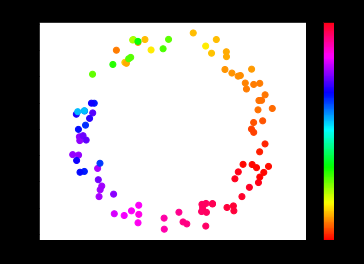
\includegraphics[scale=0.33]{pasted4} 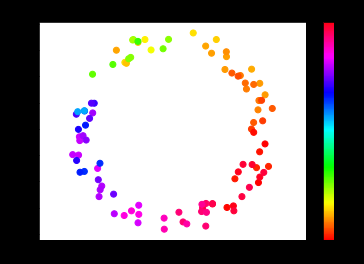
\includegraphics[scale=0.33]{pasted6}\\
\end{center}
\end{itemize}
\end{frame}
%
\begin{frame}{Another Example}
\begin{itemize}
	\item Example 2: Annulus with thin and thick parts, L2 norm ($\|f-\delta z\|_{2}$) and L1 norm ($\|f-\delta z\|_{1}$)\\
	\begin{center}
		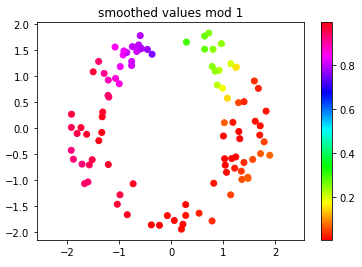
\includegraphics[scale=0.5]{thin_anulus_l2}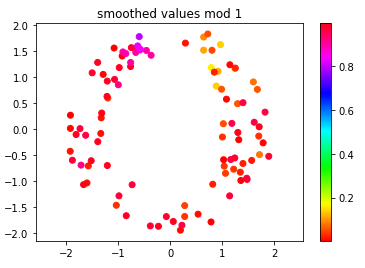
\includegraphics[scale=0.5]{thin_anulus_l1}\\
	\end{center}
\end{itemize}
\end{frame}

\begin{frame}{Another Example}
\begin{itemize}
\item Example 3: Double Annulus, mixed L2 and L1 norm ($(1-\lambda)\|f-\delta z\|_{L^{2}}+\lambda\|f-\delta z\|_{L^{1}}$) with $\lambda\in[0,1]$.\\
\begin{center}
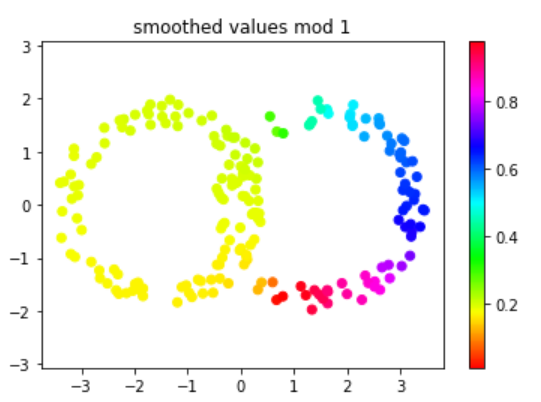
\includegraphics[scale=0.66]{DoubleAnn}
\end{center}
\end{itemize}
\end{frame}

\end{document}
